%----------------------------------------------------------------------------------------
%	PACKAGES AND OTHER DOCUMENT CONFIGURATIONS
%----------------------------------------------------------------------------------------
\documentclass[12pt,a4paper]{report}
\usepackage[english]{babel}
\usepackage[utf8x]{inputenc}
\usepackage{amsmath}
\usepackage{graphicx}
\usepackage{float}
\usepackage[colorinlistoftodos]{todonotes}
\usepackage{listings}
\usepackage{xcolor}
\usepackage{tikz}
\usepackage{fancyhdr}
\usepackage{titlesec}
\usepackage{tocloft}
\usepackage{subcaption}
\usepackage[a4paper,top=3cm,bottom=2cm,left=3cm,right=3cm,marginparwidth=1.75cm]{geometry}

% Define custom colors
\definecolor{codegreen}{HTML}{50C878}
\definecolor{codegray}{HTML}{808080}
\definecolor{codepurple}{HTML}{A020F0}
\definecolor{backcolour}{HTML}{F5F5F5}

% Define code listing settings
\lstset{
    backgroundcolor=\color{backcolour},
    commentstyle=\color{codegreen},
    keywordstyle=\color{magenta},
    numberstyle=\tiny\color{codegray},
    stringstyle=\color{codepurple},
    basicstyle=\ttfamily\footnotesize,
    breakatwhitespace=false,
    breaklines=true,
    captionpos=b,
    keepspaces=true,
    numbers=left,
    numbersep=5pt,
    showspaces=false,
    showstringspaces=false,
    showtabs=false,
    tabsize=2
}

\renewcommand{\thesection}{\arabic{section}}
\renewcommand{\cftsecfont}{\bfseries}
\titleformat{\section}[block]{\normalfont\Large\bfseries}{\thesection}{1em}{}
\setlength{\parindent}{0pt}

%----------------------------------------------------------------------------------------
%	COVER
%----------------------------------------------------------------------------------------

\begin{document}

\begin{titlepage}

    \newcommand{\HRule}{\rule{\linewidth}{0.5mm}}

    \center
    \vspace*{1.5cm}

    %----------------------------------------------------------------------------------------
    %	HEADING SECTIONS
    %----------------------------------------------------------------------------------------

    
\includegraphics[scale=.2]{src/cuhk.png}\\[1cm]
    \textsc{\large The Chinese University of Hong Kong, Shenzhen}\\[1.5cm]

    %course code
    \textsc{\Large Course Code}\\[0.5cm]

    %course name
    \textsc{\large Course Name}\\[0.5cm]

    %----------------------------------------------------------------------------------------
    %	TITLE SECTION
    %----------------------------------------------------------------------------------------

    \HRule \\[0.4cm]
    { \huge \bfseries Your Title}
    \HRule \\[1.5cm]

    %----------------------------------------------------------------------------------------
    %	AUTHOR SECTION
    %----------------------------------------------------------------------------------------

    \begin{minipage}{0.4\textwidth}
        \begin{tabular}{l l}
            \emph{Author:\quad}     & Your Name       \\
            \emph{Student ID:\quad} & Your Student ID \\
        \end{tabular}

    \end{minipage}\\[2cm]

    %----------------------------------------------------------------------------------------
    %	DATE SECTION
    %----------------------------------------------------------------------------------------

    % Date
    {\large \today}\\[2cm]
    \vfill
\end{titlepage}

%----------------------------------------------------------------------------------------
%	CONTENTS
%----------------------------------------------------------------------------------------

\tableofcontents
\newpage

%----------------------------------------------------------------------------------------
%	HEADER AND FOOTER
%----------------------------------------------------------------------------------------

\fancypagestyle{mypagestyle}{
    \fancyhf{}
    \fancyhead[L]{\small Your Title}
    \fancyhead[R]{\small Your Student ID}
    \fancyfoot[C]{\thepage} % Add this line to include page numbers at the center of the footer
    \renewcommand{\headrulewidth}{1pt}
}

% Apply custom page style
\pagestyle{mypagestyle}

%----------------------------------------------------------------------------------------
%	MAIN BODY
%----------------------------------------------------------------------------------------

\section{Part 1}

This is an example code listing:

% Code listing
\begin{lstlisting}[language=C++, caption=Example C++ code]
printf("Hello, world!")
\end{lstlisting}

\subsection{Subsection 1}
This is a subsection.

% Figure
\begin{figure}[h]
    \centering
    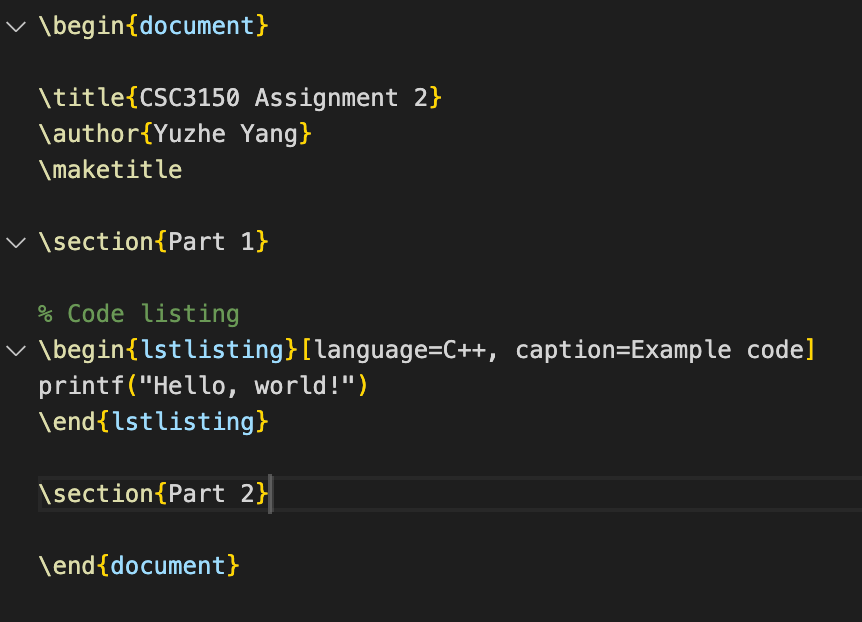
\includegraphics[width=0.3\textwidth]{src/example.png}
    \caption{Example image}
\end{figure}

\subsection{Subsection 2}
%Subfigure
\begin{figure}[h]
    \centering

    \begin{subfigure}{0.4\textwidth}
        \centering
        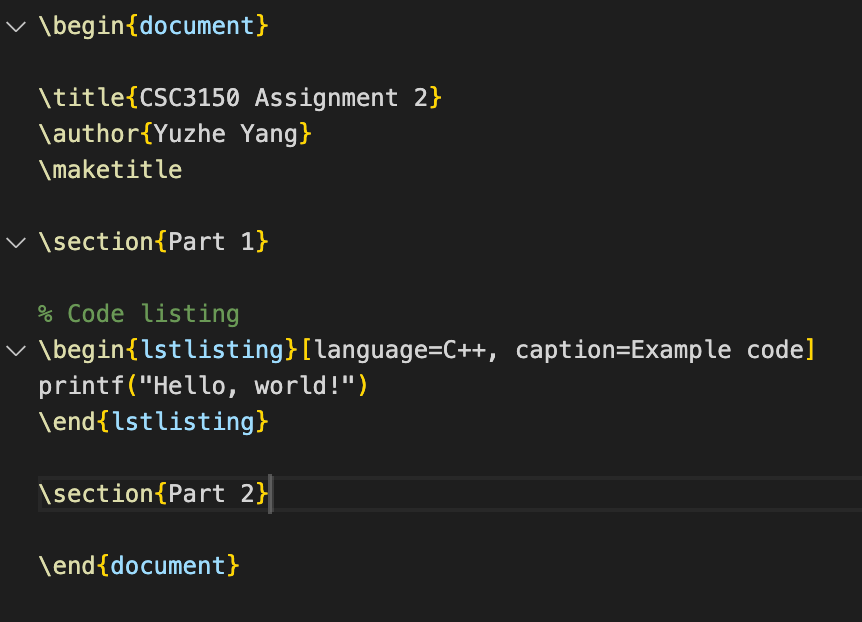
\includegraphics[width=\textwidth]{src/example.png}
        \caption{Caption for Image 1}
    \end{subfigure}
    \hfill
    \begin{subfigure}{0.4\textwidth}
        \centering
        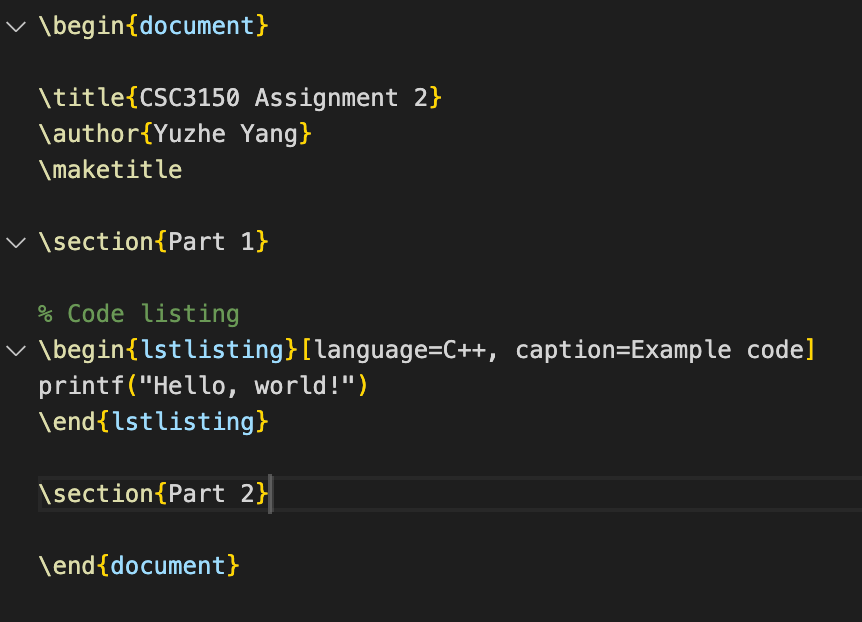
\includegraphics[width=\textwidth]{src/example.png}
        \caption{Caption for Image 2}
    \end{subfigure}

    \vspace{0.5cm} % adjust vertical space between rows

    \begin{subfigure}{0.4\textwidth}
        \centering
        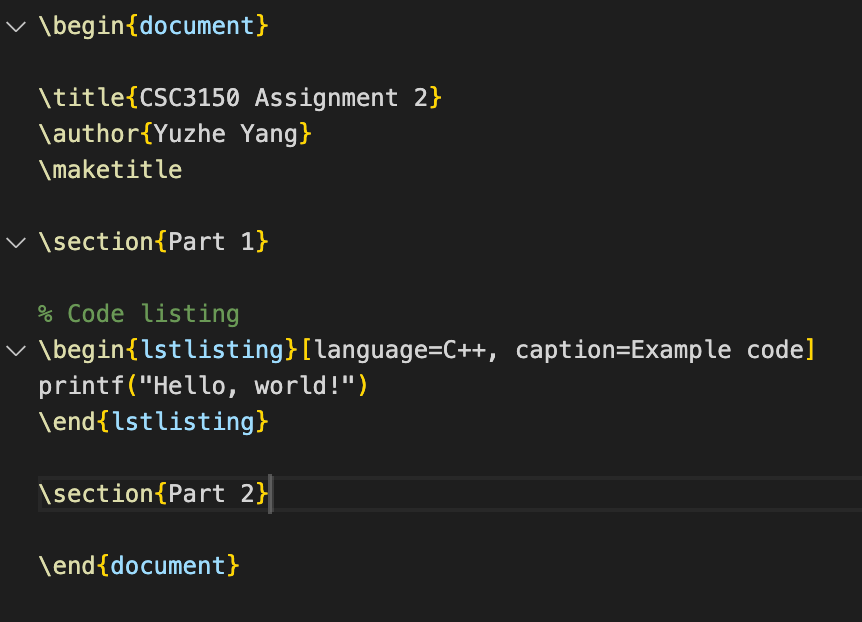
\includegraphics[width=\textwidth]{src/example.png}
        \caption{Caption for Image 3}
    \end{subfigure}
    \hfill
    \begin{subfigure}{0.4\textwidth}
        \centering
        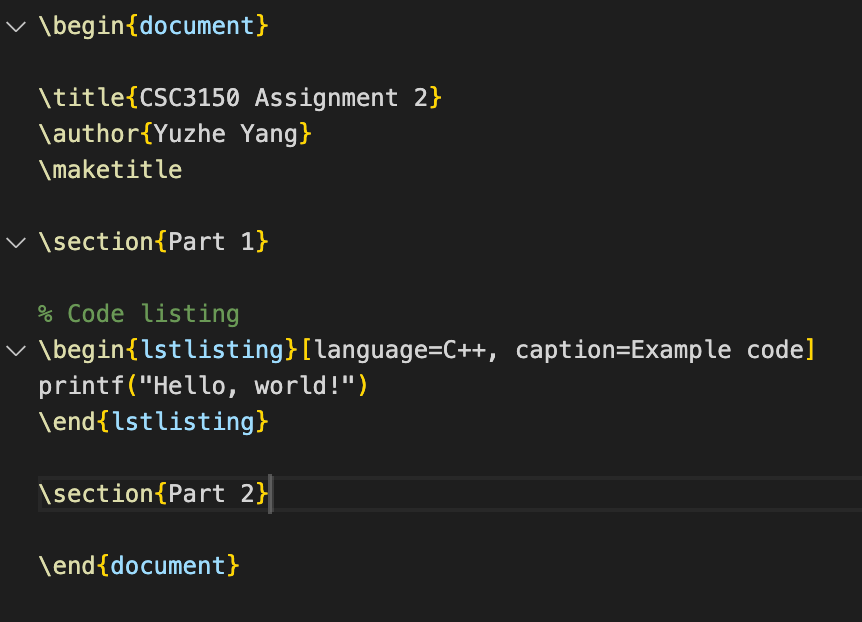
\includegraphics[width=\textwidth]{src/example.png}
        \caption{Caption for Image 4}
    \end{subfigure}

    \caption{Example of the 2x2 Image Grid}
\end{figure}

\section{Part 2}
This is an example of an inline equation: $\int_{0}^{1} x^2 dx = \frac{1}{3}$.

This is an example of a displayed equation:
\begin{equation}
    \int_{0}^{1} x^2 dx = \frac{1}{5}
\end{equation}

% Graph
This is an example graph:
\begin{center}
    \begin{tikzpicture}[scale=0.7]
        \draw[->] (0,0) -- (5,0) node[right] {$x$};
        \draw[->] (0,0) -- (0,5) node[above] {$y$};
        \draw[scale=0.5,domain=0:4,smooth,variable=\x,blue] plot ({\x},{\x*\x});
        \node[below] at (2, -1) {$y = x^2$};
    \end{tikzpicture}
\end{center}

\section{Part 3}
% Table
\begin{table}[h]
    \centering
    \begin{tabular}{|c|c|c|}
        \hline
        \textbf{Column 1} & \textbf{Column 2} & \textbf{Column 3} \\
        \hline
        Row 1, Column 1   & Row 1, Column 2   & Row 1, Column 3   \\
        \hline
        Row 2, Column 1   & Row 2, Column 2   & Row 2, Column 3   \\
        \hline
        Row 3, Column 1   & Row 3, Column 2   & Row 3, Column 3   \\
        \hline
    \end{tabular}
    \caption{Example table}
\end{table}

\end{document}